\section{Conservatively Approaching the Orchestration Problem}

\mnote{Optimal orchestration unachievable}
In the preceding section, we have proven undecidability of the orchestration problem, and we have discussed that it is unlikely to find a practical restriction of the problem such that it becomes decidable.
In consequence, we cannot achieve optimality of an orchestration and application function, which results in an 
algorithm that does not return optimal results and, depending on its implementation, may even not terminate.
Since the algorithm cannot return optimal results anyway, termination can at least be achieved by introducing an artificial upper bound for the number of executed transformation.
This potentially prevents the algorithm from finding consistent orchestrations in even more cases.

\mnote{Gradual optimality notion}
Based on those insights, we assume in this section that the orchestration problem cannot be restricted such that it becomes decidable.
We accept that any application function and any algorithm that realizes it will only realize a conservative approximation of the orchestration problem.
This means that it may only return consistent models delivered by a consistent orchestration, but it may not find a consistent orchestration although it exists.
Considering consistent orchestrations as \emph{positives}, we say that the function or algorithm, respectively, may deliver \emph{false negatives} but no \emph{false positives} and call it \emph{conservative}.
We investigate how we can define optimality of the application function in a gradual rather than a binary way, which is supposed to indicate how likely it is that it finds a consistent orchestration.
We then follow the goal of finding means to systematically improve optimality.
Since there are always cases in which the algorithm does not find a consistent orchestration, we propose an algorithm that is supposed to help identifying the reasons for failing in such cases in the subsequent section.

% \begin{itemize}
%     \item We conclude that we need to deal with the situation of undecidability. In consequence, orchestration must operate conservatively, i.e., we cannot assume to always find a solution, but if find it, it must be consistent.
%     \item One approach could be to reduce conservativeness. But even if we reduced conservativeness, we would not be able to completely eliminate it and thus have to deal with the situation that the strategy does not find a solution although it may exist.
%     \item We thus propose an approach that helps to identify the reason when the strategy is in the conservative case, i.e., not able to find a solution although it exists.
% \end{itemize}

%We found that we cannot achieve optimality (undecidability) for arbitrary transformations, we cannot restrict transformation such that we achieve decidability and thus optimality.
%So, we need to deal with situation can we cannot resolve all networks.
%Conclude: Conservativeness rather than correctness or achieving optimality (but improving the latter one)

% \mnote{Achieving a correct application function}
% The definition of the application function basically ensures that the function either returns $\bot$ or executes the \modellevelconsistencypreservationrules given by the orchestration function to retrieve a changes tuple of models.
% It is considered \emph{correct} if it ensures that its result is either $\bot$ or a consistent model tuple by executing the \modellevelconsistencypreservationrules given by the orchestration function.
% % A correct application function thus has to ensure that its result is either $\bot$ or a consistent model tuple by executing the \modellevelconsistencypreservationrules given by the orchestration function.
% In consequence, the application function can be realized by simply executing the result of the orchestration function and check whether the resulting model tuple is consistent or not and return an appropriate result.
% Such a realization is generic and does not depend on the actual consistency preservation rules and orchestration function but represents a generic behavior.
% Additionally, this gives an implementation of that function the ability to present a faulty result to the user, which eases finding out why no consistent state was reached.

% \mnote{Correctness is not crucial}
% Finally, correctness is not crucial, because correctness can easily be achieved by performing any execution of transformations and just ensuring that we terminate at some point in time and then decide whether the resulting models are consistent or not and appropriately deliver the result.

% \mnote{How to define an orchestration function that is as optimal as possible?}
% The remaining difficulty is how to define an orchestration function that fulfills the definition, i.e., to find a finite sequence of transformations, and also one that improves optimality, as an \emph{optimal} function can never be given.
% Although the definition of the orchestration function proposes a closed description of that function, in practice such a function will not have a closed form but will be realized as an algorithm that dynamically decides which transformation to execute next.
% Therefore the arising problem is that the length of the sequence to execute is not known a priori. Therefore, we need some abortion criterion. When a consistent result is found, this criterion is easy. But since we do not know whether a sequence exist, we need an abortion criterion that is reasonable and does not cut off the process although a consistent solution could be found, thus reducing optimality.
% A simple realization for that algorithm to deliver a finite sequence of transformations would be to define a fixed termination criterion, such as a specific number of transformation executions. However, there is no upper bound for the number of executed transformations necessary to achieve consistency. Still, a fixed number (even 0) could be defined for the number of executed transformations to fulfill the definition. Hence, optimality would be 0 then as a consistent result is never reached. We therefore discuss in the following how to define an appropriate orchestration function and how to optimize it.


\subsection{Systematic Improvement of Optimality}
\label{chap:orchestration:conservative:improvement}

%\subsection{A Gradual Notion of Optimality}
%\subsection{Reducing Conservativeness}

%Due to Turing-completeness of the network this would mean that the orchestration function can decide whether a Turing machine halts, which is proven impossible.
%Thus, our only goal can be to achieve optimality as far as possible in terms of reducing the degree of conservativeness, i.e., reduce the cases in which no sequence is found although it exists.

\mnote{Gradual optimality notion}
Since no optimal application function can be achieved, we can at least define a gradual notion of optimality.
It indicates for how many inputs of models and changes the application function is able to return consistent models in comparison to the number of cases in which a consistent orchestration exists at all.
This can be seen as a fitness function for the optimality $\function{Opt}$ of an application function:
\begin{align*}
    &
    \function{Opt}(\appfunction{\orcfunction{\transformationset{T}}}) \\
    & \formulaskip
    \equalsperdefinition 
    \frac{
        \abs{\setted{%\modeltuple{m} \in \metamodeltupleinstanceset{M},\changetuple{\metamodeltuple{M}} \in \changeuniverse{\metamodeltuple{M}}} 
        \tupled{\modeltuple{m},\changetuple{\metamodeltuple{M}}} \mid \appfunction{\orcfunction{\transformationset{T}}}(\modeltuple{m}, \changetuple{\metamodeltuple{M}}) \mathtextspacearound{is consistent to} \transformationset{T}}}
    }{
        \abs{\setted{\tupled{\modeltuple{m},\changetuple{\metamodeltuple{M}}} \mid \mathtextspaceafter{consistent orchestration of} \transformationset{T} \mathtextspacearound{exists for} \tupled{\modeltuple{m}, \changetuple{\metamodeltuple{M}}}}}
    }
\end{align*}

\mnote{Concrete optimality values irrelevant}
In fact, the numerator and denominator will usually both have infinite values, as there is an infinite number of possible models and changes to them.
It does, however, not matter for us what the actual optimality value of an application function is.
The purpose of the formula is only to explicitly state the influencing factors of optimality to discuss its systematic improvement.

\mnote{Average probability for finding consistent orchestration}
Obviously, we may only improve the numerator to improve optimality, because the denominator, i.e., the number of cases in which consistent orchestrations exist, depends only on the transformations and not the application function.
%is, first, not easy to achieve, and, second, may also reduce the number of cases in which a consistent orchestration is found.
How to improve the numerator highly depends on the actually implemented application and orchestration functions.
For the most general case, let us assume that we have an application function $\appfunction{\orcfunction{\transformationset{T}}}$ whose orchestration function randomly determines any orchestration, i.e., it selects one of all possible orchestrations according to an equal distribution.
So we consider the following event $E_{\modeltuple{m},\changetuple{\metamodeltuple{M}}}$:
\begin{align*}
    &
    E_{\modeltuple{m},\changetuple{\metamodeltuple{M}}}: \appfunction{\orcfunction{\transformationset{T}}}(\modeltuple{m}, \changetuple{\metamodeltuple{M}}) \mathtextspacearound{is consistent to} \transformationset{T}
\end{align*}
The probability that this event occurs is given by the ratio between the number of consistent orchestrations for that input and the number of all orchestrations:
\begin{align*}
    &
    P(E_{\modeltuple{m},\changetuple{\metamodeltuple{M}}}) = \frac{
        \abs{\setted{\sequence{\transformation{t}} \in \transformationset{T}^{< \mathbb{N}} \mid \sequence{\transformation{t}} \mathtextspacearound{is consistent orchestration for} \tupled{\modeltuple{m}, \changetuple{\metamodeltuple{M}}}}}
    }{
        \abs{\transformationset{T}^{< \mathbb{N}}}
    }
\end{align*}
Here, the denominator is the size of what we previously introduced as the problem space $P = \abs{\transformationset{T}^{< \mathbb{N}}}$ containing all possible orchestrations, and the numerator is the size of what we previously introduced as the solution space $S_{\modeltuple{m}, \changetuple{\metamodeltuple{M}}} = \abs{\setted{\sequence{\transformation{t}} \in \transformationset{T}^{< \mathbb{N}} \mid \sequence{\transformation{t}} \mathtextspacearound{is consistent orchestration for} \tupled{\modeltuple{m}, \changetuple{\metamodeltuple{M}}}}}$, which contains all consistent orchestrations for an input of models and changes.

\mnote{Expected value for finding consistent orchestration}
We can introduce a stochastic variable $AppCons_{\modeltuple{m},\changetuple{\metamodeltuple{M}}}$, which assigns the values $0$ and $1$ to the events $E_{\modeltuple{m},\changetuple{\metamodeltuple{M}}}$ and its complementary:
\begin{align*}
    AppCons_{\modeltuple{m},\changetuple{\metamodeltuple{M}}}(\omega) \equalsperdefinition 
    \begin{cases}
        0, & \omega = \appfunction{\orcfunction{\transformationset{T}}}(\modeltuple{m}, \changetuple{\metamodeltuple{M}}) \mathtextspacearound{is not consistent to} \transformationset{T} \\
        1, & \omega = \appfunction{\orcfunction{\transformationset{T}}}(\modeltuple{m}, \changetuple{\metamodeltuple{M}}) \mathtextspacearound{is consistent to} \transformationset{T}
    \end{cases}
\end{align*}
The expected value of this variable is then equal to the probability of the event $E_{\modeltuple{m},\changetuple{\metamodeltuple{M}}}$ to occur:
\begin{align*}
    \mu(AppCons_{\modeltuple{m},\changetuple{\metamodeltuple{M}}}) = P(AppCons_{\modeltuple{m},\changetuple{\metamodeltuple{M}}} = 1) = P(E_{\modeltuple{m},\changetuple{\metamodeltuple{M}}})
\end{align*}

\mnote{Number of found consistent orchestration}
For an application function that chooses a random orchestration, we can thus express the numerator of $\function{Opt}(\appfunction{\orcfunction{\transformationset{T}}})$ as the sum of expected values of the stochastic variables for all possible inputs.
\begin{align*}
    &
    \abs{\setted{\tupled{\modeltuple{m},\changetuple{\metamodeltuple{M}}} \mid \appfunction{\orcfunction{\transformationset{T}}}(\modeltuple{m}, \changetuple{\metamodeltuple{M}}) \mathtextspacearound{is consistent to} \transformationset{T}}} = \sum_{\modeltuple{m},\changetuple{\metamodeltuple{M}}} \mu(AppCons_{\modeltuple{m},\changetuple{\metamodeltuple{M}}}) \\
    & \formulaskip
    = \frac{
        \sum_{\modeltuple{m},\changetuple{\metamodeltuple{M}}} \abs{\setted{\sequence{\transformation{t}} \in \transformationset{T}^{< \mathbb{N}} \mid \sequence{\transformation{t}} \mathtextspacearound{is consistent orchestration for} \tupled{\modeltuple{m}, \changetuple{\metamodeltuple{M}}}}}
    }{
        \abs{\transformationset{T}^{< \mathbb{N}}}
    }
\end{align*}

\mnote{Improvement by reducing considered orchestrations}
Thus, if we can increase $P(E_{\modeltuple{m},\changetuple{\metamodeltuple{M}}})$, we also improve optimality, even if orchestrations are chosen randomly.
We can increase this probability by either improving the number of consistent orchestrations or by reducing the number of possibly considered orchestrations.
The number of consistent orchestrations can only be influenced by requirements to the transformations.
For example, the requirement of consistency relations to be compatible improves these values, as we have shown by example in \autoref{chap:compatibility}.
In the following, we discuss how we can reduce the number of possibly considered orchestrations while not reducing the number of consistent orchestrations, thus improving the probability of the application function to find a consistent orchestration and thus improving optimality.

\begin{figure}
    \centering
    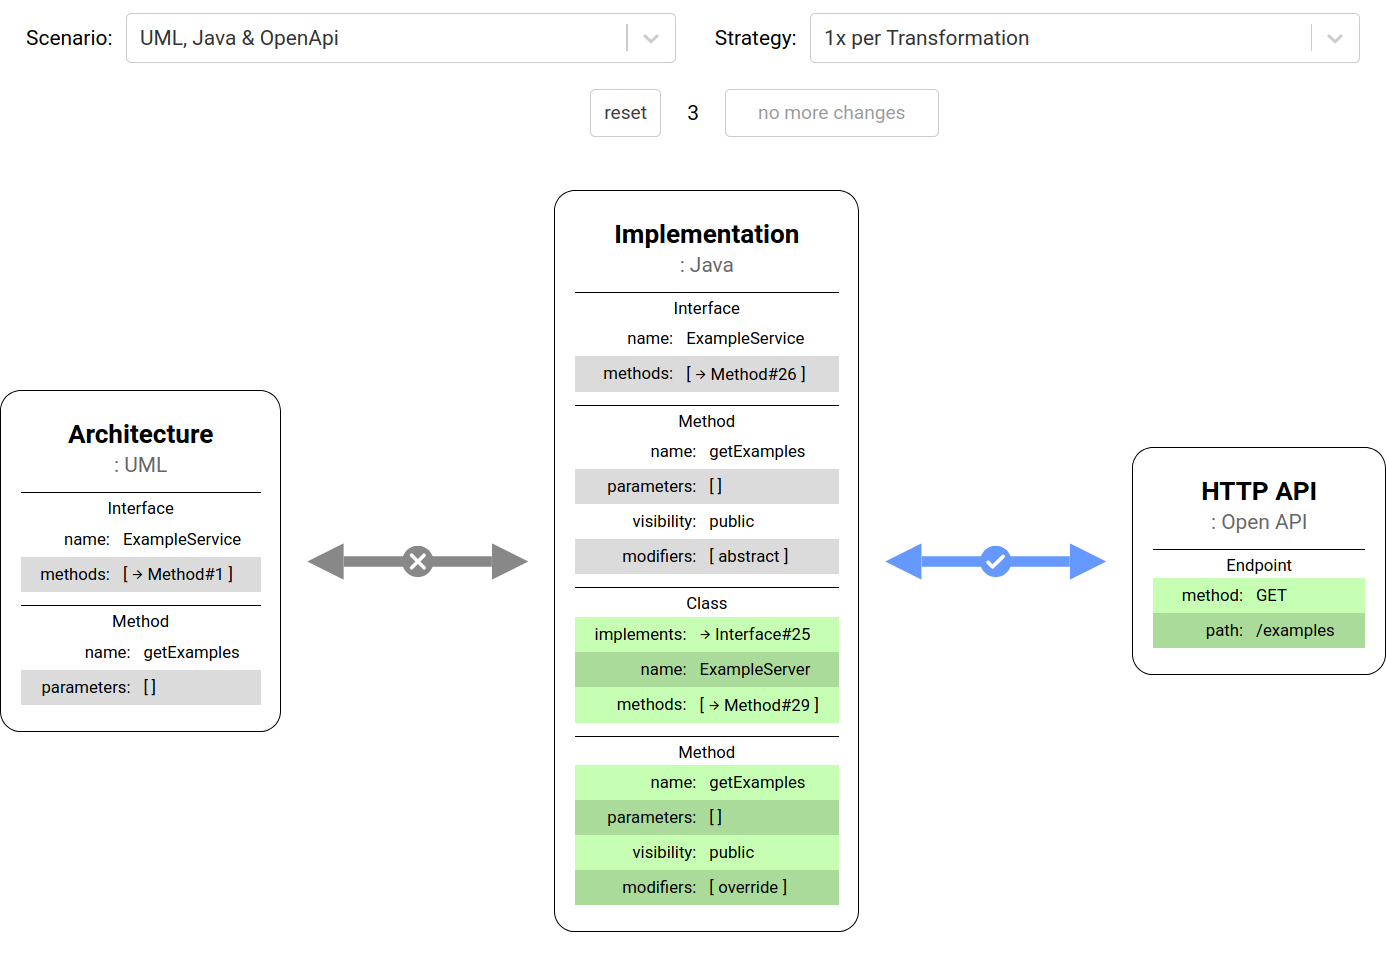
\includegraphics[width=\textwidth]{figures/correctness/orchestration/simulator_screenshot.png}
    \caption[Screenshot of the transformation network simulator]{Screenshot of a network of for an architecture specification, its implementation, and an \gls{API} specification in OpenAPI~\cite{OpenAPI}, which requires multiple execution of the same transformation, developed in the transformation network simulator~\cite{gleitze2020OrchestrationSimulator}.}
    \label{fig:orchestration:simulator}
\end{figure}

\mnote{No systematic improvement}
The application function can, of course, contain more intelligent logic for determining an orchestration beyond the random selection of transformations to improve the number of cases in which it finds a consistent orchestration.
By implementing further mechanisms to make a reasonable selection, the possibility to find a consistent orchestration may be further improved.
We investigated different orchestration strategies, such as the depth-first or breadth-first selection of transformations in the induced graph, and analyzed them with a simulator developed specifically for that purpose, which is available at GitHub~\cite{gleitze2020OrchestrationSimulator}.
An example of a scenario showing the necessity to execute transformation more than once that we implemented in the simulator is depicted in \autoref{fig:orchestration:simulator}
For each strategy, however, we found categories of transformation networks for which it performed worse than some other strategy.

\mnote{Backtracking to explore problem space}
Another strategy could be to try different orchestrations as soon as it turns out that one orchestration cannot yield consistent models.
This can, for example, be achieved by performing backtracking.
\autoref{algo:orchestration:application} dynamically selects transformations to execute. 
Thus, as soon as the algorithm detects that no further transformation executions can lead to a consistent orchestration, it can revert the last transformation execution and proceed with another transformation.
This means that it resets the state of generated changes and executed transformations to the one before the current execution of the orchestration loop and proceeds again with another transformation.
If all transformations as continuations of one sequence of executed transformations have been tried out, the algorithm recursively steps back the iterations of the loop.
While this approach, in theory, allows us to explore the complete problem space $P = \transformationset{T}^{< \mathbb{N}}$, it is impractical because the problem space is infinitely large.
It may, however, be used to try different options in a subset of the problem space, for example, those with a limited length.

% We need to deal with the situation that no consistent orchestration exists and that we are not able to find it, even if it exists, as the problem space is arbitrarily large (arbitrary high number of transformation executions).
% This forbids approaches such as backtracking to find an appropriate solution.
% \todo{Discuss Backtracking}

\mnote{Avoiding alternation}
Since we did not find a strategy that is, in general, superior to other investigated strategies, we gave up that direction and focused on finding orchestrations that should be generally avoided.
To this end, we consider alternation as a possibility to reduce the number of cases in which non-termination can occur, thus improving optimality by both its dynamic detection and its avoidance.
%Additionally, we have focused on finding a strategy that improves the ability to deal with the fact that an optimality of~$1$ can never be achieved such that the process of finding the reason for not finding a consistent orchestration is supported.

% In fact, both these numbers usually infinite, an there is an infinite number of possible models and deltas. However, it does finally not matter for us what the actually value is, but only how to improve that value.
% \todo{We have to map that value to compatibility, which reduces the number of potential false orders.}

% \textbf{Overall Goal:} Find correct orchestration function that improves optimality.

% There are two ways to improve optimality of the orchestration function:
% \begin{enumerate}
%     \item Optimize the orchestration function, i.e., find a good order (probably this is not possible), at least find an order that helps the developer to find problems
%     \item Optimize the input, i.e., define requirements to the transformations and their relations representing the input to optimize optimality
% \end{enumerate}
% \todo{We need an example for that}

% Both goes hand in hand, because restrictions to the input can never lead to an orchestration function that always terminates without leading to unsupported relevant cases.

% This conform to two approaches:
% \begin{enumerate}
%     \item Dynamic decision about selected transformation and abortion criteria
%     \item Constructive restrictions that ensure that appropriate order is (easily) found
% \end{enumerate}

%\todo{Application function can be generically defined, orchestration maybe not? We actually want to ensure that both are generic and none of them has to be defined for a specific project.}

%\subsection{Systematic Improvement of Optimality}
%\paragraph{Avoidance of Non-Termination}

% In consequence, we propose to dynamically deal with alternation / divergence.
% To detect alternations, the execution can simply track if a state way already processed. Apart from spatial problems, this does always work.
% Finding divergence is not that easy, because it is generally not possible to define an upper bound for the number of executions of a single transformation.
% This is due to the reason that, again, this conflicts with the Halting problem.
% We can see this at the simple example in \autoref{fig:formal:noupperboundexample}.

% \begin{figure}
%     \centering
%     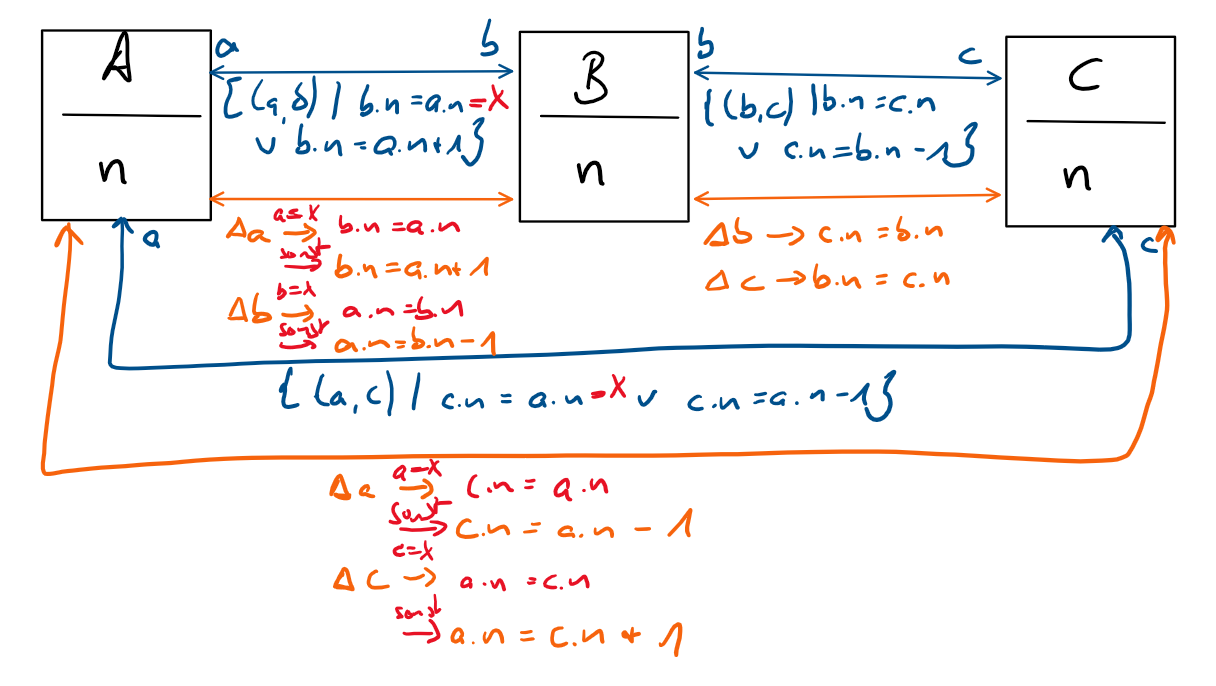
\includegraphics[width=\textwidth]{figures/correctness/orchestration/no_upper_bound_example_old.png}
%     \caption{Example for no upper bound}
%     \label{fig:formal:noupperboundexample}
% \end{figure}

% Depending on the value X, the transformations have to be executed X times to result in a consistent state. This value can be arbitrarily chosen, thus an arbitrary number of executions may be necessary to terminate in a consistent state.

% \todo{Moved from single execution section -> revise}
% \begin{theorem}[Orchestration with Unbounded Executions]
%     \label{theorem:unbounded_execution}
%     For any set of transformations $\transformationset{T}$, there can be models $\modeltuple{m}$ and changes $\changetuple{}$ to them for which each possible orchestration function $\orcfunction{\transformationset{T}}$ with whom $\appfunction{\orcfunction{\transformationset{T}}}(\modeltuple{m}, \changetuple{})$ is consistent, such that $\abs{\orcfunction{\transformationset{T}}(\modeltuple{m}, \changetuple{})} > \abs{\transformationset{T}}$.
% \end{theorem}
% \begin{proof}
%     We know from \autoref{lemma:minimal_executions} that $\transformationset{T}_{inc}$ requires at least $4$ executions of $\transformation{t}_{12}$ for the inputs defined in \autoref{lemma:minimal_executions} when selecting $x \geq 5$.
%     Thus, for any orchestration function, we know that $\abs{\orcfunction{\transformationset{T}}(\modeltuple{m}, \changetuple{})} > 4 > 3 = \abs{\transformationset{T}_{inc}}$.
%     This proves the theorem by example.
% \end{proof}


\subsection{Dynamic Detection of Alternation} % Divergence and alternation
\label{chap:orchestration:conservative:alternation}

\mnote{Orchestration requires abortion criterion}
The proposed algorithm, like any algorithm, is supposed to \emph{terminate} in a specific \emph{state} to be considered correct.
In our case, such a correct state, as required by an application function it implements, is the return of consistent models or $\bot$, which the algorithm fulfills by construction.
In particular, the algorithm does never return models that are inconsistent, neither because it does not detect that they are inconsistent nor because it detects that they are inconsistent but still returns them.
From our previous findings regarding decidability, we know that we cannot expect the algorithm to realize an optimal application function.
Thus, we either need to implement \function{Orchestrate} such that it always returns $\bot$ after a finite number of executions to ensure termination, which results in returning $\bot$ although an order of transformations could yield consistent models, or we allow an arbitrary number of executions to improve the ability to find consistent results but accept that the algorithm may not terminate.

\mnote{Definition of alternation}
We have discussed that non-termination of the algorithm can occur because no consistent orchestration exists at all or because the algorithm is not able to find it.
A special case of non-termination is \emph{alternation}, which means that the same states are passed repeatedly. 
In case of transformation networks, alternation means that from some point in time the subsequent executions of the transformations in Line~\ref{algo:orchestration:application:line:stepcalculation} of \autoref{algo:orchestration:application} repeatedly produce the same sequence of results, i.e., of changes.
% Non-termination can, in general, manifest in terms of \emph{alternation} or \emph{divergence}, which means that either the same states are passed repeatedly or that an infinite sequence of different states is produced.
% In case of transformation networks, alternation means from some point in time the subsequent executions of the transformations in Line~\ref{algo:orchestration:application:line:stepcalculation} of \autoref{algo:orchestration:application} repeatedly produce the same sequence of results, i.e., of changes.
% Divergence means that from some point in time all results, i.e., changes, produced in Line~\ref{algo:orchestration:application:line:stepcalculation} differ.
In contrast to non-termination in general, the scenario of alternation can at least be avoided by construction.
% To this end, the history of change produced by the algorithm in Line~\ref{algo:orchestration:application:line:stepcalculation} has to be stored.
% It can either be used by the \function{Apply} function to detect alternation or by passing it to the \function{Orchestrate} function to influence the selection of transformations to avoid alternation.

\begin{definition}[Alternation of Apply Algorithm]
    \label{def:applyalternation}
    During an execution of \autoref{algo:orchestration:application}, let there be a number $n$ of executions of the transformation execution loop in Lines~\ref{algo:orchestration:application:line:startorchestrate}--\ref{algo:orchestration:application:line:endorchestrate} of \autoref{algo:orchestration:application}, such that for all numbers of loop executions $> n$ there is a sequence of executed transformations and generated changes that occur subsequently at the end of the current states of $\applyalgexecuted$ and $\applyalggenerated$ at least two times.
    Then we call the execution of the algorithm \emph{alternating}.
    If the execution of the algorithm does not terminate and is not alternating, we call it \emph{diverging}.
\end{definition}

\mnote{Orchestrate function detecting alternation}
The \function{Orchestrate} function receives the history of transformations and already generated changes, and is thus able to identify the situation that the same sequence of transformations was already executed and produced equal changes with each application.
This allows to implement the function in a way that it does not return the same sequence of transformations when it was already passed and produced the same changes, e.g., by performing backtracking if such a situation is detected.
If a concrete realization of the \function{Orchestrate} function is not implemented in a way that it can react to the detection of alternation and produce a different sequence of transformations, it can at least return $\bot$ to ensure termination of \function{Apply}, because repeated execution of the same transformations will still return the same changes. 

\mnote{Avoiding alternation improves orchestration}
Alternation produces orchestrations that can never yield consistent models, thus they are part of the problem space $P = {\transformationset{T}^{< \mathbb{N}}}$ of finding an orchestration for a given input $i$ of models and changes but can never be part of the solution space $S_{\modeltuple{m}, \changetuple{\metamodeltuple{M}}} = \abs{\setted{\sequence{\transformation{t}} \in \transformationset{T}^{< \mathbb{N}} \mid \sequence{\transformation{t}} \mathtextspacearound{is consistent orchestration for} \tupled{\modeltuple{m}, \changetuple{\metamodeltuple{M}}}}}$ containing the consistent orchestrations.
Avoiding such alternations thus reduces the problem space without affecting the solution space and thus improves the possibility to find a consistent orchestration, as shown in the previous subsection.

%Divergence: If it passes the same changes again, then it either does not pass those changes again 

% Derive from the previous insights that whenever the algorithm does not terminate, we can have two situations: divergence and alternation.
% Prove that no other options for occurring situation exist!

% Problemraum:
% \begin{itemize}
%     \item Ziel ist, dass ein Netzwerk von Transformationen nach einer Änderung in einem konsistenten Zustand terminiert. D.h. Korrektheit stellt Anforderungen an \emph{Terminierung}, sowie den \emph{Zustand} bei Terminierung.
%     \item Folgende Abweichungen davon können auftreten:
%     \begin{enumerate}
%         \item Nicht-Terminierung: Das Netzwerk terminiert nicht. Das bedeutet im Prinzip, dass die Ausführungsfunktion (bzw. der Laufzeit-Algorithmus, der die Funktion dynamisch emuliert) nicht \emph{sound} ist. Soundness der Ausführungsfunktion setzt voraus, dass die berechnet Aufrufsequenz endlich ist. Wenn die Ausführung nicht terminiert, bedeutet das, dass entweder die gleichen Zustände mehrfach durchlaufen werden oder eine Sequenz unendlich vieler Zustände produziert wird. Denn wenn beides nicht der Fall ist, gibt es eine endliche Sequenz unterschiedlicher Zustände, d.h. Terminierung. Das bedeutet, dass es folgende zwei Möglichkeiten gibt:
%         \begin{itemize}
%             \item Alternierung: Die gleichen Zustände werden mehrfach durchlaufen.
%             \item Divergenz: Es werden unendlich viele Zustände produziert.
%         \end{itemize}
%         \item Inkonsistente Terminierung: Die Ausführungsfunktion bzw. der Algorithmus beendet die Ausführung, aber in einem inkonsistenten Zustand. Hier lassen sich ebenfalls wieder zwei Fälle unterscheiden.
%         \begin{itemize}
%             \item Unerkannte Inkonsistenz: Der Algorithmus terminiert und denkt, der Zielzustand wäre konsistent. Dies bedeutet aber direkt, dass nicht alle Konsistenzrelationen erfüllt sind, was, zumindest in der Theorie, einfach zu prüfen wäre (entweder durch Prüfung der Relationen oder durch Ausführung der hippokratischen Transformationen, die alle nichts tun dürften)
%             \item Erkannte Inkonsistenz: Der Algorithmus terminiert, wissend dass die Lösung nicht konsistent ist. Dies kann entweder sein, weil eine Transformation für zwei Modelle in einem inkonsistenten Zustand nicht mehr anwendbar ist, oder weil irgendein anderes Abbruchkriterium erreicht ist.
%         \end{itemize}
%     \end{enumerate}
% \end{itemize}

% Assume we have an algorithm that sequentially applies transformations.
% It stops as soon as a transformation cannot be applied or the models are consistent.
% Then we need to guarantee termination.
% We need to avoid that transformations can be applied indefinitely never leading to consistent models.

% Reasons for this situation are alternation and divergence.
% Prove that if we do not pass the same model state again (alternation) and if there is no indefinite number of model states (divergence), the algorithm terminates.
% Thus, if we ensure that any execution order of transformations does never lead to alternation and divergence, we know that the algorithm terminates!!

% \begin{itemize}
%     \item Zeigen, dass es Beispiele gibt, in denen es unabhängig von der Ausführungsreihenfolge immer zu einer Alternierung kommt
%     \item Zeigen, dass es Beispiele gibt, in denen es unabhängig von der Ausführungsreihenfolge immer zu einer Divergenz kommt.
%     \item Die Beispiele sollten zeigen, dass wir keine Einschränkungen an die Transformationen machen können, was das Problem aushebelt. D.h. egal welche Einschränkungen ich an die Transformationen definiere, es lassen sich immer Beispiele konstruieren, in denen es keine Ausführungsreihenfolge gibt, in denen sie terminieren.
%     \item Mathematisch zeigen, dass Alternierung und Divergenz die einzigen Probleme sind. D.h. wenn nicht der gleiche Zustand mehrmals durchlaufen wird (Alternierung) und es nicht unendlich viele Zustände gibt (Divergenz), dann ist die Folge endlich.
%     %\item Außerdem mathematisch die Abbildung von Transformationen auf Turing-Maschinen zeigen und damit ableiten, dass allgemeine Netzwerke erstmal nicht terminieren müssen (Abbildung auf Halteproblem)
% \end{itemize}

% To avoid these problems by construction, we discussed before that we need to achieve that P = S, such that the application function can execute transformations in an arbitrary order to achieve consistency.

% Another possibility would be to allow the problems and detect them dynamically and react to them.
% We will finally discuss that in the last section.

%In the following, we discuss whether and how we may restrict synchronizing transformations, such that an arbitrary execution order can avoid divergence and alternation, such that the algorithm terminates.


\subsection{Monotony for Avoiding Alternation}

\mnote{Non-alternation by construction}
We have discussed %in \autoref{chap:orchestration:conservative:alternation}
that alternation of \autoref{algo:orchestration:application}, as a specific kind of non-termination scenario, can be avoided by construction of the orchestration function or at least can be detected by the \function{Apply} algorithm.
Instead of detecting alternation during orchestration, we may also restrict the transformation network such that no alternation can occur by construction.
We can achieve this by defining a notion of monotony for the transformations.

\mnote{Monotony notion from synchronizing transformations}
For the construction of synchronizing bidirectional transformations by unidirectional consistency preservation rules in \autoref{chap:synchronization:bidirectional:transformations}, we have defined the property of \emph{partial consistency improvement}, which is a monotony notion for the two unidirectional consistency preservation rules of a synchronizing bidirectional transformation, as each execution of them improves that property.
We can, however, not define monotony in a similar way for the whole transformation network for two reasons.
First, the notion of partial consistency is not applicable to transformation networks, because each transformation needs to restore consistency between two models completely.
Second, since each transformation is developed independently from all others, we cannot apply the notion of partial consistent improvement to the other models by restricting how far a transformation may violate consistency to the other transformations.
%
We thus define the following, different notion of monotony for transformations.
\begin{definition}[Monotone Synchronizing Transformation]
    \label{def:monotonetransformation}
    Let $\metamodeltuple{M} = \tupled{\metamodelsequence{M}{n}}$ be metamodels and let $\transformation{t}$ be a synchronizing transformation. We call $\transformation{t}$ monotone if, and only if, it does not change elements that were already changed:
    \begin{align*}
        &
        \forall \modeltuple{m} = \tupled{\model{m}{1}, \dots, \model{m}{n}} \in \metamodeltuple{M}, \changetuple{\metamodeltuple{M}} = \tupled{\change{\metamodel{M}{1}}, \dots, \change{\metamodel{M}{n}}} \in \changeuniverse{\metamodeltuple{M}} : \\
        & \formulaskip
        \bigl(
        \exists \changetuple{\metamodeltuple{M}}' = \tupled{\change{\metamodel{M}{1}}', \dots, \change{\metamodel{M}{n}}'} \in \changeuniverse{\metamodeltuple{M}} : \generalizationfunction{\metamodeltuple{M},\transformation{t}}(\modeltuple{m}, \changetuple{\metamodeltuple{M}}) = (\modeltuple{m},\changetuple{\metamodeltuple{M}}') \\
        & \formulaskip
        \Rightarrow
        % WE CANNOT ASSUME TRANSFORMATION TO BE STRONG MONOTONE, BECAUSE IF TRANSFORMATION IS EXPECTED FOR ALREADY CONSISTENT MODELS, IT CANNOT CHANGE ANYTHING
        % (\changetuple{\metamodeltuple{M}}'(\changetuple{\metamodeltuple{M}}(\modeltuple{m})) = \changetuple{\metamodeltuple{M}}(\modeltuple{m}) \Rightarrow \modeltuple{m} \consistenttomath \transformationset{T}) \\
        % & \formulaskip
        % \land 
        \forall i \in \setted{1, \dots, n} : 
        (\change{\metamodel{M}{i}}(\model{m}{i}) \setminus \model{m}{i}) \subseteq \change{\metamodel{M}{i}}'%(\change{\metamodel{M}{i}}
        (\model{m}{i})%) 
        \\
        & \formulaskip\formulaskip
        \land
        (\model{m}{i} \setminus \change{\metamodel{M}{i}}(\model{m}{i})) \cap \change{\metamodel{M}{i}}'%(\change{\metamodel{M}{i}}
        (\model{m}{i})%)
         = \emptyset)
        \bigr)
        %\change{\metamodeltuple{M}}(\modeltuple{m}) \subseteq \modeltuple{m} \cup \changetuple{\metamodeltuple{M}}'(\changetuple{\metamodeltuple{M}}(\model{m}{}))
        %\land
        %\modeltuple{m} \cup \changetuple{\metamodeltuple{M}}'(\changetuple{\metamodeltuple{M}}(\model{m}{})) \subseteq \changetuple{\metamodeltuple{M}}(\model{m}{})\big)
    \end{align*}
\end{definition}

\mnote{No repeated change of same elements}
The definition is based on the idea that transformations are only supposed to append changes but not to revert previous changes.
This means that elements that were introduced by previous changes still need to be present after applying the transformation.
Additionally, elements that were removed are not allowed to be added by the transformation again.
Thus, all elements of the originally changed models were either contained in the original models or are contained in the models yielded by the transformation execution, which leads to the model relations in the definition.

% \begin{definition}[Strongly Monotone Synchronizing Transformation]
%     Let $\metamodeltuple{M}$ be metamodels and let $\transformation{t}$ be a monotone synchronizing transformation. We call $\transformation{t}$ strongly monotone if it does not perform any changes only when all models are already consistent does not change elements that were already changed, i.e.
% \end{definition}

\mnote{Property of monotone transformation orchestrations}
Having only monotone transformations ensures that the application of each orchestration that does not apply a transformation to already consistent models yields a sequence of pairwise different model states.
\begin{lemma}[Monotone Transformation Orchestration Prefixes]
    \label{lemma:monotonetransformationsnosamestates}
    Let $\transformationset{T}$ be a set of correct monotone synchronizing transformations for a tuple of metamodels $\metamodeltuple{M}$.
    Then for all models and changes, as well as any orchestration $\sequenced{\transformation{t}_{1}, \dots, \transformation{t}_{m}} \in \transformationset{T}^{< \mathbb{N}}$ that does not contain a transformation to be executed when its models are already consistent, the prefixes of that orchestration only yield the same models if those prefixes are consistent orchestrations:
    \begin{align*}
        &
        \forall \modeltuple{m} \in \metamodeltupleinstanceset{M}, \changetuple{\metamodeltuple{M}} \in \changeuniverse{\metamodeltuple{M}} : \forall i, k \in \setted{1, \dots, m} : \\
        &
        \generalizationfunction{\metamodeltuple{M}, \transformation{t}_{i}} \concatfunction \dots \concatfunction \generalizationfunction{\metamodeltuple{M}, \transformation{t}_{1}}(\modeltuple{m}, \changetuple{\metamodeltuple{M}}) = \generalizationfunction{\metamodeltuple{M}, \transformation{t}_{k}} \concatfunction \dots \concatfunction \generalizationfunction{\metamodeltuple{M}, \transformation{t}_{1}}(\modeltuple{m}, \changetuple{\metamodeltuple{M}}) \\
        & \formulaskip 
        \Rightarrow
        \exists \changetuple{\metamodeltuple{M}}' \in \changeuniverse{\metamodeltuple{M}} :
        \generalizationfunction{\metamodeltuple{M}, \transformation{t}_{k}} \concatfunction \dots \concatfunction \generalizationfunction{\metamodeltuple{M}, \transformation{t}_{1}}(\modeltuple{m}, \changetuple{\metamodeltuple{M}}) = (\modeltuple{m}, \changetuple{\metamodeltuple{M}}') \\
        & \formulaskip\formulaskip
        \land 
        \changetuple{\metamodeltuple{M}}'(\modeltuple{m}) \consistenttomath \transformationset{T}
        \end{align*}
\end{lemma}
\begin{proof}
    Assume that there are two prefixes $\sequenced{\transformation{t}_{1}, \dots, \transformation{t}_{i}}$ and $\sequenced{\transformation{t}_{1}, \dots, \transformation{t}_{k}}$ of an orchestration, $i < k$ without loss of generality, such that they yield the same inconsistent models, i.e., $\generalizationfunction{\metamodeltuple{M}, \transformation{t}_{i}} \concatfunction \dots \concatfunction \generalizationfunction{\metamodeltuple{M}, \transformation{t}_{1}}(\modeltuple{m}, \changetuple{\metamodeltuple{M}}) = \generalizationfunction{\metamodeltuple{M}, \transformation{t}_{k}} \concatfunction \dots \concatfunction \generalizationfunction{\metamodeltuple{M}, \transformation{t}_{1}}(\modeltuple{m}, \changetuple{\metamodeltuple{M}})$ although $\generalizationfunction{\metamodeltuple{M}, \transformation{t}_{k}} \concatfunction \dots \concatfunction \generalizationfunction{\metamodeltuple{M}, \transformation{t}_{1}}(\modeltuple{m}, \changetuple{\metamodeltuple{M}})$ is not consistent to $\transformationset{T}$.
    We denote the change tuple delivered by any prefixes of length $l$ as $\changetuple{\metamodeltuple{M},l} = \tupled{\change{\metamodel{M}{1},l}, \dots, \change{\metamodel{M}{n}, l}}$ with $(\modeltuple{m}, \changetuple{\metamodeltuple{M},l}) = \generalizationfunction{\metamodeltuple{M}, \transformation{t}_{l}} \concatfunction \dots \concatfunction \generalizationfunction{\metamodeltuple{M}, \transformation{t}_{1}}(\modeltuple{m}, \changetuple{\metamodeltuple{M}})$.
    We know that the sequence of changes between the two prefixes does not perform any changes and thus acts like the identity function, i.e., %$\generalizationfunction{\metamodeltuple{M}, \transformation{t}_{k}} \concatfunction \dots \concatfunction \generalizationfunction{\metamodeltuple{M}, \transformation{t}_{i+1}}(\modeltuple{m}, \changetuple{\metamodeltuple{M},i}) = (\modeltuple{m},\identitychange(\modeltuple{m}, \changetuple{\metamodeltuple{M},i}))$
    %and thus 
    $\changetuple{\metamodeltuple{M},i}(\modeltuple{m}) = \changetuple{\metamodeltuple{M},k}(\modeltuple{m})$.
    We also know that all the transformations between the prefixes, i.e., all transformations $\transformation{t}_{l}$ for each $l$ with $i < l \leq k$, do not act like the identity function for their inputs, i.e., $\generalizationfunction{\metamodeltuple{M}, \transformation{t}_{l}}(\modeltuple{m}, \changetuple{\metamodeltuple{M},l-1}) \neq (\modeltuple{m}, \changetuple{\metamodeltuple{M},l-1})$.
    %$\generalizationfunction{\metamodeltuple{M}, \transformation{t}_{l}}(\modeltuple{m}, \changetuple{\metamodeltuple{M},l-1}) \neq (\modeltuple{m}, \identitychange(\modeltuple{m}, \changetuple{\metamodeltuple{M},l-1}))$.
    Otherwise, the models affected by the transformation would either have been consistent before, which conflicts with the assumption that the orchestration does not contain a transformation when its models are already consistent, or they would not be consistent afterwards, which conflicts with the assumed correctness of the transformations.

    Thus, each transformation $\transformation{t}_{l} \; (i < l \leq k)$ performs modifications to the change tuple, i.e., adds or removes further elements.
    This especially applies to $\transformation{t}_{i+1}$.
    Let us assume that $\transformation{t}_{i+1}$ adds an element (analogous argumentation for the removal).
    %modifies the change tuple such that it adds or removes further elements.
    Then there is a model that contains the element after applying the change generated by the transformation, i.e., $\exists s \in \setted{1, \dots, n} : \exists \modelelement{e} : \modelelement{e} \in \change{\metamodel{M}{s},i+1}(\model{m}{s}) \setminus \change{\metamodel{M}{s},i}(\model{m}{s})$.
    Due to the transformations being monotone, we know that this element was not contained before, especially not in $\model{m}{s}$, as otherwise $\modelelement{e} \in \model{m}{s} \setminus \change{\metamodel{M}{s},i}(\model{m}{s})$ and thus $(\model{m}{s} \setminus \change{\metamodel{M}{s},i}(\model{m}{s})) \cap \change{\metamodel{M}{s},i+1}(\model{m}{s}) \neq \emptyset$, which conflicts the definition of monotone transformations for $\transformation{t}_{i+1}$.

    Since $\change{\metamodel{M}{s},k}(\model{m}{s}) = \change{\metamodel{M}{s},i}(\model{m}{s})$, we know that $\modelelement{e} \not\in \change{\metamodel{M}{s},k}(\model{m}{s})$.
    Thus, there must be a transformation $\transformation{t}_{l}$ with $i+1 < l \leq k$ which, in turn, removes this element, i.e., $\modelelement{e} \in \change{\metamodel{M}{s},l-1}(\model{m}{s}) \setminus \change{\metamodel{M}{s},l}(\model{m}{s})$.
    Then $\modelelement{e} \in \change{\metamodel{M}{s},l-1}(\model{m}{s}) \setminus \model{m}{s}$ and thus $\change{\metamodel{M}{s},l-1}(\model{m}{s}) \setminus \model{m}{s} \not\subseteq \change{\metamodel{M}{s},l}(\model{m}{s})$, which conflicts the definition of monotone transformations for $\transformation{t}_{l}$.

    In consequence, each transformation $\transformation{t}_{l} \; (i < l \leq k)$ can neither add nor remove an element, thus our assumption that there are two prefixes that yield the same inconsistent models does not hold, which proves the lemma.
\end{proof}

\mnote{Monotone transformation prevent alternation}
With that insight, it is easy to see that given only monotone transformations, no alternation can occur in \autoref{algo:orchestration:application}.
\begin{theorem}[Monotone Transformations Alternation Prevention]
    Let $\transformationset{T}$ be a set of correct, monotone synchronizing transformations.
    Then the execution of \autoref{algo:orchestration:application} cannot be alternating according to \autoref{def:applyalternation}, as long as $\function{Orchestrate}$ does not return a transformation whose models are already consistent.
\end{theorem}
\begin{proof}
    According to \autoref{lemma:monotonetransformationsnosamestates}, monotone transformations ensure that in an orchestration that does not contain transformations that need to be applied to already consistent models the application of two prefixes never yields the same changes.
    In consequence, the sequence of $\applyalggenerated$ in the transformation execution loop in 
    Lines~\ref{algo:orchestration:application:line:startorchestrate}--\ref{algo:orchestration:application:line:endorchestrate} of \autoref{algo:orchestration:application} can never contain the same two changes.
    This would, however, be necessary to fulfill \autoref{def:applyalternation} for alternation.
\end{proof}

\mnote{Stronger guarantee than non-alternation}
In fact, the guarantee of not producing the same state twice is even stronger than non-alternation, because alternation allows to pass the same state multiple times, as long as the same sequence of states is not passed repeatedly and infinitely.
It does, however, only make sense to pass the same state twice if the orchestration algorithm, which selects the next transformation to execute, is able to process that situation by trying different execution orders if an alternation occurs.
Thus, the less strict requirement for alternation is suited to make statements about the orchestration strategy but not about the individual transformations, as it is unlikely to find a property for a single transformation that gives a guarantee that depends on the execution order of transformations, like alternation does.

\mnote{Monotony generally not assumable}
Monotone transformations guarantee non-alternation, but monotony according to \autoref{def:monotonetransformation} is not a property that we can assume to be fulfilled by all transformations.
Although it seems intuitive that a transformation should not remove elements that were added before and vice versa, this does also mean that, for example, an attribute value may only be changed once by the transformations.
This would, however, require the transformations to always make a choice for attributes that fits for all other transformations as well.
We have seen in different examples, such as the one depicted in \autoref{fig:orchestration:no_upper_bound} and \autoref{fig:orchestration:no_orchestration}, that it may be necessary to change elements multiple times, because the transformations select values with which the models only fulfill their own consistency relation but not those of the other transformations.
It may take several executions to find a value selection with which the models are consistent to all transformations.
We might say that the transformations need to \emph{negotiate} a consistent solution.

\mnote{Ensuring monotony as often as possible}
Still, the given examples were rather artificial and are not an indicator for monotony to be practically unachievable.
It may, at least in some cases, be possible to specify monotone transformations.
Even if only some of the transformations or only specific rules of them are monotone, it improves the chance that an orchestration strategy finds a consistent orchestration.
Having the knowledge about the benefits of monotony gives a transformation developer the ability to implement it as often as possible.

\mnote{Combining alternation avoidance and detection}
Finally, the possibility to avoid alternation by construction can be combined with the ability of an orchestration strategy to react to alternation.
We have discussed in \autoref{chap:orchestration:conservative:alternation} that an orchestration strategy can detect alternation and adapt its strategy of selecting the next transformation in that case.
In addition, if monotony is given at least for some transformations, the orchestration strategy needs to try less execution orders and thus improves the chance of finding a consistent orchestration.

% \begin{figure}
%     \centering
%     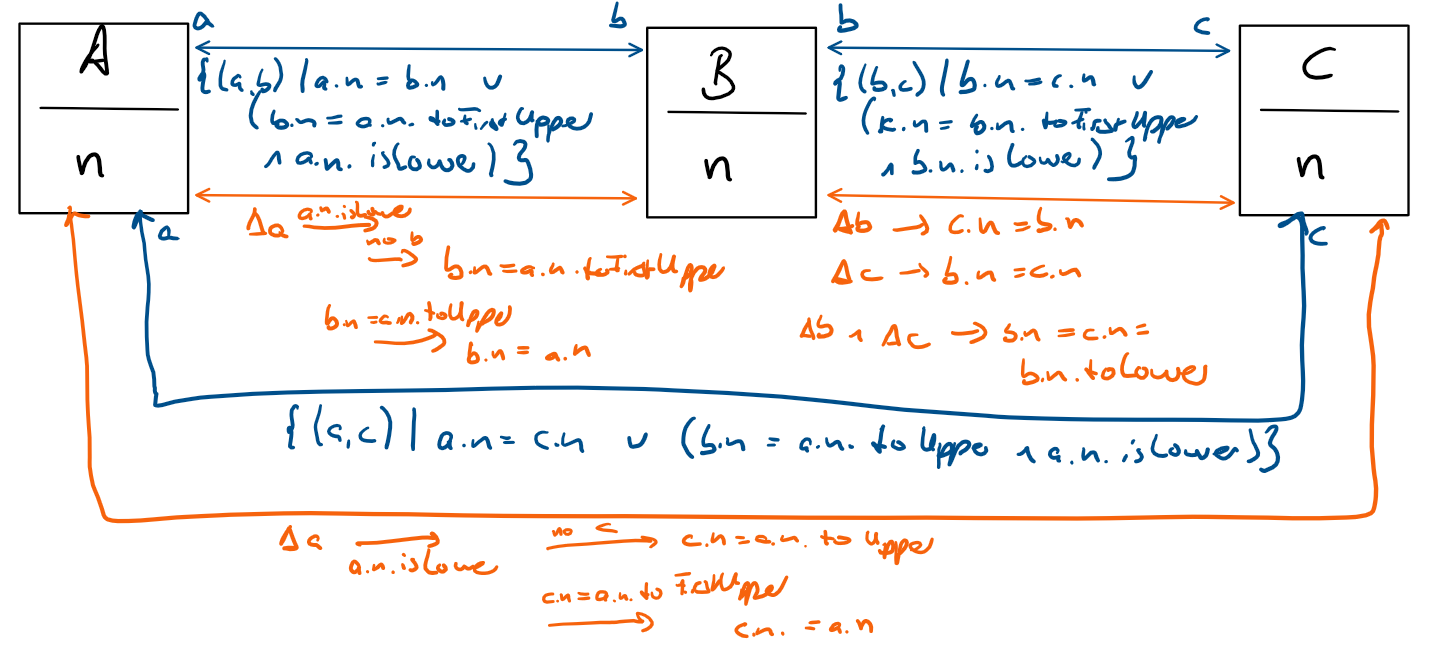
\includegraphics[width=\textwidth]{figures/correctness/orchestration/monotony_counterexample.png}
%     \caption{Counterexample for monotony}
%     \label{fig:formal:monotonycounterexample}
% \end{figure}

% \begin{itemize}
%     \item Muss eine Transformation mit jedem beliebigen Delta umgehen können müssen? Eine Einschränkung auf Monotonie würde dies verhindern. Bzw. wir müssten zeigen, dass es Konsistenzrelationen gibt, die unter der Anforderung an Monotonie nicht wiederhergestellt werden können. Bspw. fügt eine andere Transformation 3 Elemente hinzu, wo zwei mit dem anderen entsprechend der Konsistenzrelationen korrelieren und somit keine Witness-Struktur aufgebaut werden kann, die Konsistenz beweist. Das lässt sich durch Hinzufügen weiterer Elemente potentiell nicht auflösen (siehe Beispiele im SoSym-Paper).
%     \item Refer to synchronization chapter, where we introduced a monotony notion based on transformations being partial-consistency-improving. Here, in contrast, the CPRs cannot be aligned, such that we cannot, for example, expect one transformation not to lead to a reduction of consistency regarding consistency relations of other, previously executed transformations.
% \end{itemize}
% \begin{itemize}
%     \item Im Allgemeinen könnte eine Transformation beliebige dieser Deltasequenzen modifizieren. Wir verlangen jedoch, dass eine Transformation nur Deltas anhängt, also die Sequenzen länger werden
%     \item Genauer beschränken wir auch, welche Sequenzen eine Transformation sehen und ändern darf, genau gesagt darf sie die Sequenzen von zwei Modellen sehen und eine davon verlängern.
%     \item Hier kommt bereits der Unterschied zu bisherigen Transformationen, denn die sehen nur Deltas an einem Modell und erzeugen Deltas an dem anderen. Das ist bei uns schon gänzlich anders. Bidirektionale Transformationen unterstützen das im Übrigen auch nicht, sondern sind nur Spezifikationen, aus denen sich Wiederherstellungsroutinen für beide Richtungen ableiten lassen (siehe Stevens 2010)
% \end{itemize}

% \paragraph{Idea:} Require monotony to avoid alternation

% We would have to relax the definition of transformation to be monotone, because if a transformation is monotone, it may only append information, but this is not always possible, as can be seen in the following example. A monotone transformation must be able to return bottom if it cannot make further changes to restore consistency to the relation.

% \begin{definition}[Monotone Transformation]
%     Transformation gets models M and deltas D and produces new deltas D'. Taking the union of the original models M and the new models D'(M), then D(M) must be a subset of that, because other elements would have been added and removed afterwards or elements would have been changes once by D and again in a different way by D'.

%     Generally, monotony could also mean that only the same complete model state is not passed twice. \todo{Why dont we do that?}
% \end{definition}

% This would mean that each transformation only appends changes, i.e., if an element was added/removed, the transformation may not do the inverse. The same applies to attribute/reference changes: if an attribute/reference was already changes it may not be changed again.
% This way, it is by design impossible to pass through the same state again. Actually, if a monotone transformation returns bottom, the network has to terminate with a failure.
% However, this is hard restriction to transformations. It leads to the fact that in some networks that actually have a simple solution no solution is found at all. This can be easily seen at the example in \autoref{fig:formal:monotonycounterexample}. In the example adding "aa" to the left model, any execution order of the transformations leads to the situation that a previous change must be revoked to result in a consistent state. However, it is possible to derive a consistent state for that input change.

% \begin{figure}
%     \centering
%     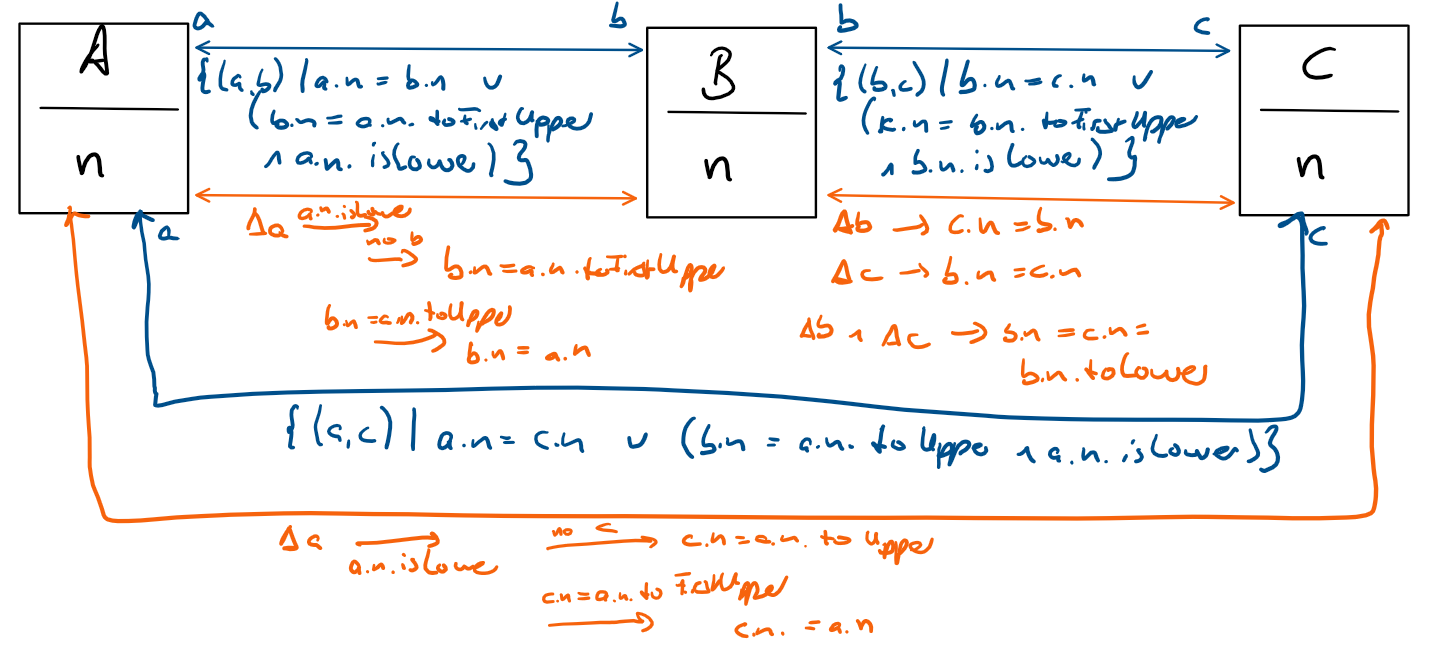
\includegraphics[width=\textwidth]{figures/correctness/orchestration/monotony_counterexample.png}
%     \caption{Counterexample for monotony}
%     \label{fig:formal:monotonycounterexample}
% \end{figure}

% One could now argue that there are binary relations in the example, which may never be fulfilled at all. We will later discuss how far relations that cannot be fulfilled should be restricted. However, in general, this is wanted behavior, because in general it may be necessary that transformations produce intermediate states that are not yet consistent with each other. Otherwise this would means that each transformation is always able to directly deliver a state that is consistent to all other relations, which is especially not possible, because other transformations may add further information to the models. More precisely, a relation may consider <a model consistent to all other models that contain any additional information not affected by the transformation. For example, a UML class model may be considered consistent to all Java models with any implementation of the specified methods, thus to an infinite number of models. Now saying that it should not be allowed that the transformation selects one with an empty implementation because that is not consistent to another relations induced by another transformation, such as the relationship to a component model, does not make any sense. Thus having those relation elements that may be considered locally consistent but will never occur in a globally consistent tuple of models does not make sense.
% In the example, we can see that such an inconsistent intermediate state is passed through and afterwards a consistent tuple of models is reached if not requiring monotony.
% In consequence, requiring monotony from transformations is a too strict requirement, because it is necessary to run through states that may be changed later on.

% \begin{theorem}
%     An application function for monotone transformations either returns a consistent model or produce a sequence of CPRs returning delta that return models of always growing size (i.e., it diverges).
% \end{theorem}

% \paragraph{Divergence cannot be avoided}

% There are rather equal network, one that terminates after a long time and one that never terminates. 
% Consider the example. The relations are defined in a way such that for any allocation for any of them a consistent tuple of models can be found. However, the transformations are not able to find it because they make "bad" choices from a set of choices that are conflicting. 
% This can be seen in the example that we have already given in \autoref{fig:correctness:no_execution_order}.

% Thus, systematically avoiding divergence is not possible. 

% \textbf{Central insight:} Alternation / Divergence cannot be avoided systematically (like in ordinary programming), if not restricting transformations in a way that may not be reasonable.


% \subsection{Unresolvability}

% Discuss why no execution order may exist although relations are compatible.
% If not even an order exists, the application function or the algorithm can, for sure, not find it.

% However, we found that we cannot always find an execution order if it exists and we were not able to find restrictions to transformations to ensure that it exists.
% We expect the same for the existence of an execution order at all.
% All restrictions we can make are likely to be too restrictive.
% The problem arises when there is an overlap of consistent models between some transformations, but they always decide for other elements that are not in the overlap of consistent models.
% It would, obviously, require the transformation to know about the others to ensure that this is not the case.
% This conflicts our assumption.

% Finally, it may be valid that for some changes no execution exists, because the change can not be processed on purpose \todo{Give example for that!}.
% Should this be the case if we assume compatibility?

% Although a more detailed investigation of the claim that we cannot define reasonable requirements to the transformations to ensure that they can always be ordered to restore consistency is a topic for further research, we did not investigate it in the scope of this thesis.
% Since we found it necessary to find a conservative algorithm that can deal with the case that no execution is found anyway, that algorithm covers the case that no execution order exists as well and thus is a solution for this problem as well.

% Beispiel:
% \begin{itemize}
%     \item Das ist im allgemeinen aber nicht Fall. Letztendlich trifft jede Transformation lokale Entscheidungen. Beispielsweise könnte jede einzelne Transformation gegeben eine beliebige Änderung immer dieselben Modelle (bzw. Änderungen die dazu führen) zurück liefern (im trivialsten Fall leere Modelle). Dann erfüllt jede Transformation ihre Korrektheitseigenschaft bzgl. ihrer Relation, aber das Netzwerk muss nicht korrekt sein, da bspw. T(A,B) und T(B,C) sich immer für verschiedene Instanzen von B entscheiden. Es gäbe somit nie eine konsistente Lösung für eine beliebige Ausführungsreihenfolge der Transformationen, auch wenn die Relationen das erlauben würden.
%     \item Beispiel mit Namen, wo eine Transformation immer den großen Namen zurück liefert, die andere immer den kleinen. T(A,B) bildet A auf gleiches B ab und beide auf kleine Schreibweise, obwohl beide erlaubt sind. Erzeuge A="a", dadurch B="a". T(B,C) bildet B auf C ab und beide auf große Schreibweise, obwohl beide erlaubt sind. Somit macht sie das zu B="A" und C="A". Nun wird T(A,B) wieder beide klein machen usw. Allerdings wäre eine insgesamt valide Lösung einfach alle groß oder alle klein zu machen, aber die Transformationen finden diesen Zustand nicht. 
% \end{itemize}
